\subsection{Two Journeys Become One: Why Vectors Add}

Suppose a point is moved twice. The first displacement is
\[
\mathbf u=(u_1,u_2),
\]
and the second is
\[
\mathbf v=(v_1,v_2).
\]
We want one vector that has exactly the same final effect as these two moves
performed successively.

\begin{corebox}[The geometric problem]
Vector addition must represent the single displacement whose effect is identical
to performing two given displacements one after the other.
\end{corebox}

\begin{derivationbox}[Coordinate form forced by successive motion]
Start at an arbitrary point $(x,y)$. After applying $\mathbf u$ we are at
\[
(x+u_1,\,y+u_2).
\]
Applying $\mathbf v$ from there gives
\[
(x+u_1+v_1,\,y+u_2+v_2).
\]
Relative to the original point, the total horizontal change is $u_1+v_1$ and
the total vertical change is $u_2+v_2$. Therefore the coordinate rule is forced
by the meaning of successive displacement.
\end{derivationbox}

\begin{definitionbox}
For vectors $\mathbf u=(u_1,u_2)$ and $\mathbf v=(v_1,v_2)$, their sum is
\[
\boxed{
\mathbf u+\mathbf v
=
(u_1+v_1,\,u_2+v_2)
}.
\]
\end{definitionbox}

\begin{interpretationbox}[What coordinatewise addition records]
The formula is bookkeeping for a journey performed in two stages. It adds
changes of the same kind: horizontal change to horizontal change and vertical
change to vertical change.
\end{interpretationbox}

\begin{center}
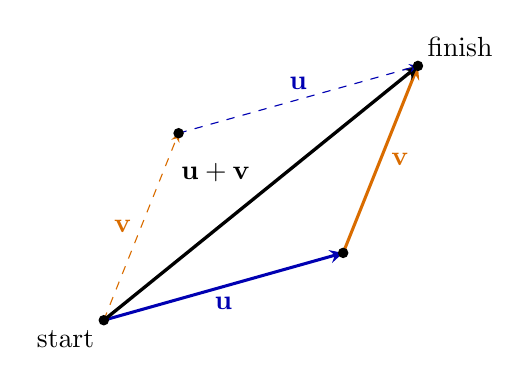
\begin{tikzpicture}[scale=0.95,>=stealth]
    \coordinate (O) at (0,0);
    \coordinate (U) at (3.2,0.9);
    \coordinate (V) at (1.0,2.5);
    \coordinate (S) at (4.2,3.4);

    \draw[blue!70!black,line width=1.1pt,->] (O) -- (U)
        node[midway,below] {$\mathbf u$};
    \draw[orange!85!black,line width=1.1pt,->] (U) -- (S)
        node[midway,right] {$\mathbf v$};
    \draw[very thick,->] (O) -- (S)
        node[midway,above left] {$\mathbf u+\mathbf v$};

    \draw[orange!85!black,dashed,->] (O) -- (V)
        node[midway,left] {$\mathbf v$};
    \draw[blue!70!black,dashed,->] (V) -- (S)
        node[midway,above] {$\mathbf u$};

    \fill (O) circle (2pt) node[below left] {start};
    \fill (U) circle (2pt);
    \fill (V) circle (2pt);
    \fill (S) circle (2pt) node[above right] {finish};
\end{tikzpicture}
\end{center}

\begin{proofbox}[Why the order does not change the result]
The diagram contains two routes to the same endpoint:
\[
\mathbf u\text{ then }\mathbf v,
\qquad
\mathbf v\text{ then }\mathbf u.
\]
They agree because addition of real numbers is commutative:
\[
u_1+v_1=v_1+u_1,
\qquad
u_2+v_2=v_2+u_2.
\]
Therefore
\[
\mathbf u+\mathbf v=\mathbf v+\mathbf u.
\]
\end{proofbox}

\begin{theorembox}
Vector addition is commutative:
\[
\boxed{\mathbf u+\mathbf v=\mathbf v+\mathbf u}.
\]
Geometrically, this is the parallelogram rule.
\end{theorembox}

Subtraction answers a different practical question: what displacement must be
performed after $\mathbf v$ in order to have the same effect as $\mathbf u$?
We seek a vector $\mathbf w$ satisfying
\[
\mathbf v+\mathbf w=\mathbf u.
\]

\begin{derivationbox}[Subtraction as the missing displacement]
Solving the equation $\mathbf v+\mathbf w=\mathbf u$ coordinate by coordinate
gives
\[
\mathbf w=(u_1-v_1,\,u_2-v_2).
\]
\end{derivationbox}

\begin{definitionbox}
For vectors $\mathbf u=(u_1,u_2)$ and $\mathbf v=(v_1,v_2)$,
\[
\boxed{
\mathbf u-\mathbf v
=
(u_1-v_1,\,u_2-v_2)
}.
\]
In particular,
\[
\boxed{\overrightarrow{AB}=B-A}.
\]
\end{definitionbox}

\begin{remarkbox}
The expression $B-A$ does not subtract geometric points as physical objects. It
subtracts their coordinate addresses to recover the displacement carrying one
point to the other.
\end{remarkbox}
